\chapter{Appendix}

%appendix
For each measurement site, a minimum of 100 force curve readings per site was taken, with the raw data saved in a single file. The full dataset is attached as a zip file for each concentration, site and parameters. Run folders correspond to approach curves, Run-ret are retract folders.

Because there are an incredible amount of images involved the dataset, the entire appendix has been provided as a comprehensive .7z file. If this 7z is missing, it's because it was too big to upload.

\section{Tip Speed Analysis Histograms}

The data used in the tip speed analysis is provided below. This is to support the  graphs in Chapter 7; fig \ref{fig:ApproachAverageSpeed} and fig\ref{fig:RetractAverageSpeed}.


% 0.6mM Section
\subsubsection*{0.6 mM}
For 0.6 mM, only one site was recorded. Interestingly, 2 Hz 0.6 mM presented the highest recorded repulsive force across the entire dataset, including 0.5 Hz 0.6 mM, which is in line with what is expected from DLVO. 

\begin{figure}[h!!!]
\centering
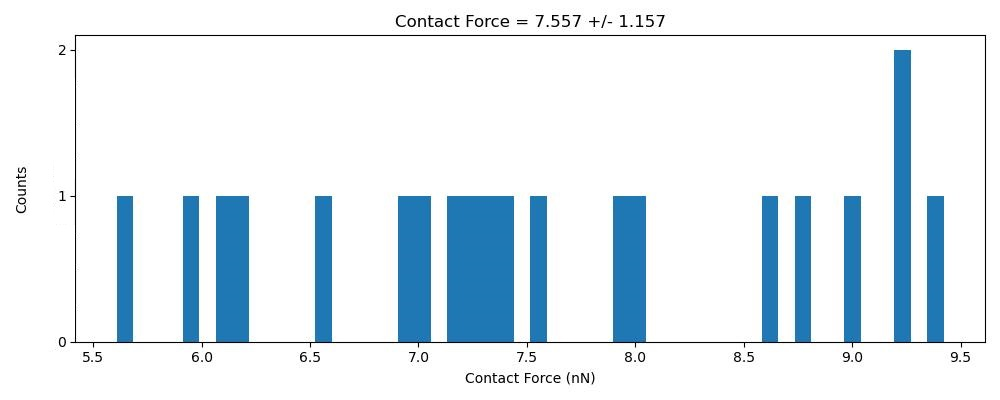
\includegraphics[width=\textwidth]{chapter7/Tip speed/0.6mM/approach_f_c_hist.jpg}
\caption{Approach force-current histogram at 0.6mM at 2Hz}
\label{fig:0.62hz.png}        
\end{figure}

\begin{figure}[h!!!]
\centering
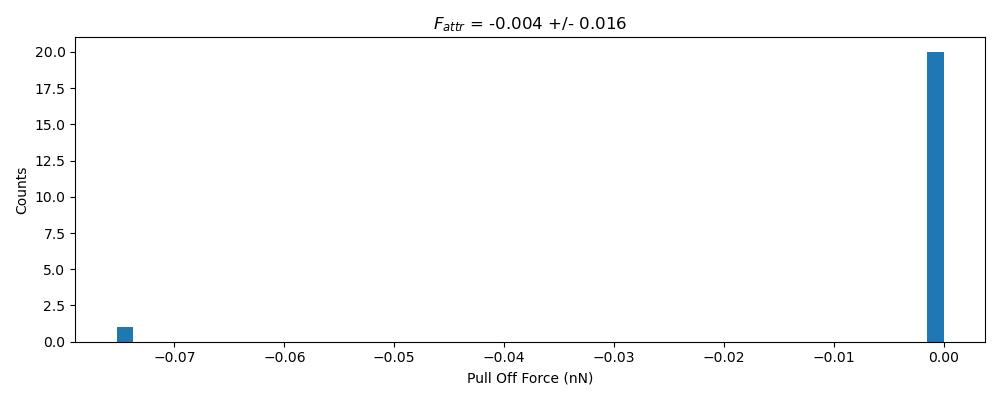
\includegraphics[width=0.9\textwidth]{chapter7/Tip speed/0.6mM/retract_f_a_hist.jpg}
\caption{Retract force-amplitude histogram at 0.6mM at 2Hz}
\end{figure}



\newpage

% 1.6mM Section
\subsubsection*{1.6mM}
1.6mM demonstrates a return to the previously expected values as set from the previous datasets. The retract curve demonstrates a widening of the attractive force, but still a very minor attraction.
\begin{figure}[h!]
\centering
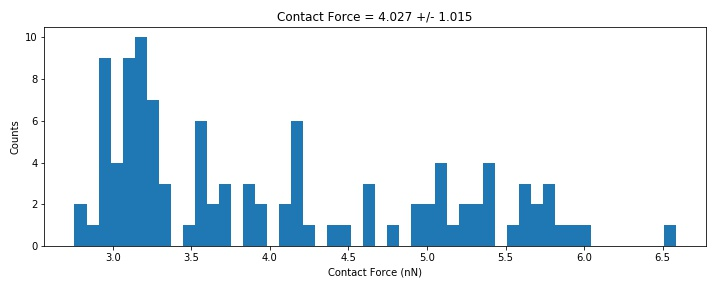
\includegraphics[width=.9\textwidth]{chapter7/Tip speed/1.6mM/S1 2Hz/approach_f_c_hist.jpg}
\caption{Approach curve for 1.6mM, S2 at 2Hz}
\end{figure}

\begin{figure}[h!]
\centering
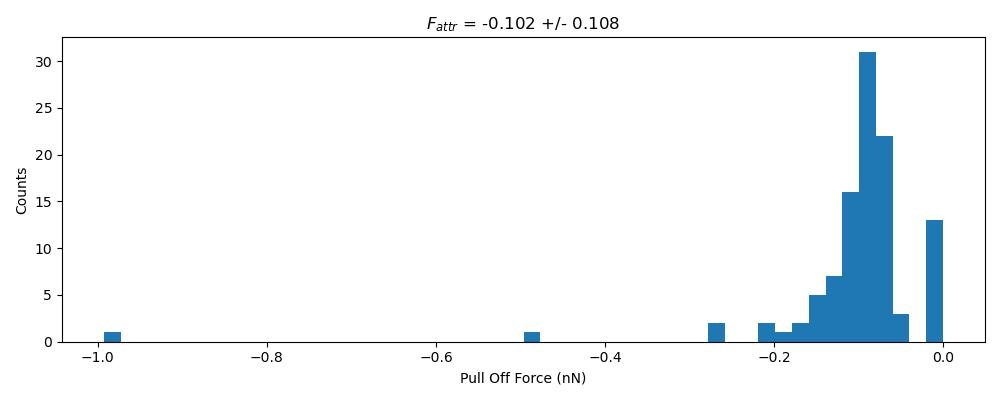
\includegraphics[width=.9\textwidth]{chapter7/Tip speed/1.6mM/S1 2Hz/retract_f_a_hist.jpg}
\caption{Retract curve for 1.6mM, S2 at 2Hz}
\end{figure}

\newpage

% 5mM Section
\subsubsection*{5mM}
5mM is the first concentration where a wider range of sites were explored. For the approach, the largest distribution was around the 2.5-4nN range, which is within expectations. For the retrace, minor instances of adhesive force was observed, but not significantly, again in line with previous results.

\begin{figure}[h!]
\paragraph{S1 2Hz}
\centering
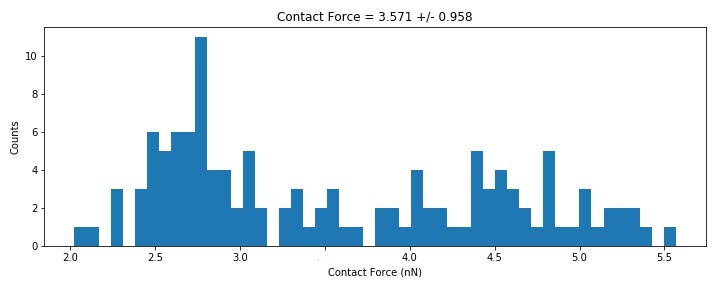
\includegraphics[width=\textwidth]{chapter7/Tip speed/5mM/S1 2Hz/approach_f_c_hist.jpg}
\caption{Approach curve for 5mM, S1 at 2Hz}
\end{figure}

\begin{figure}[h!]
\centering
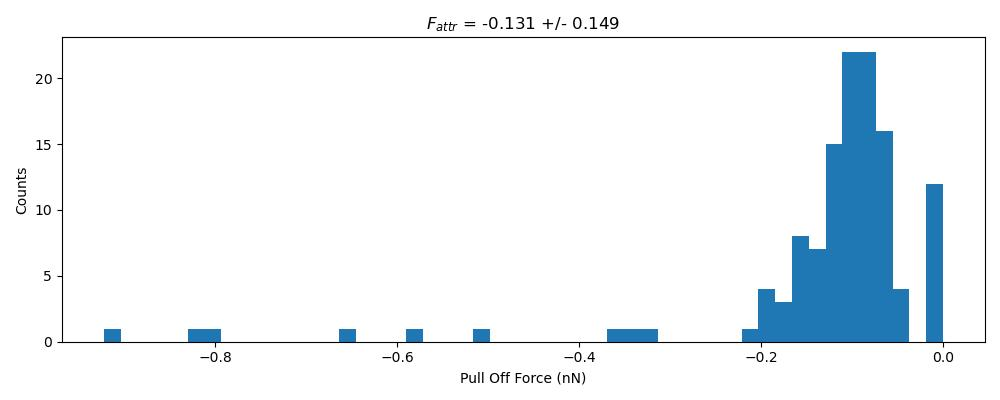
\includegraphics[width=\textwidth]{chapter7/Tip speed/5mM/S1 2Hz/retract_f_a_hist.jpg}
\caption{Retract curve for 5mM, S1 at 2Hz}
\end{figure}
\newpage


\begin{figure}[h!]
\paragraph{S2 2Hz}
\centering
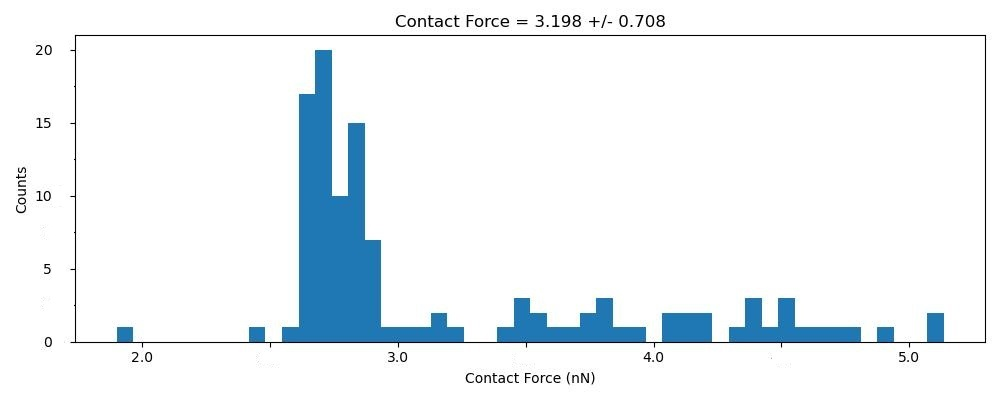
\includegraphics[width=\textwidth]{chapter7/Tip speed/5mM/S2 2Hz/approach_f_c_hist.jpg}
\caption{Approach curve for 5mM, S2 at 2Hz}
\end{figure}

\begin{figure}[h!]
\centering
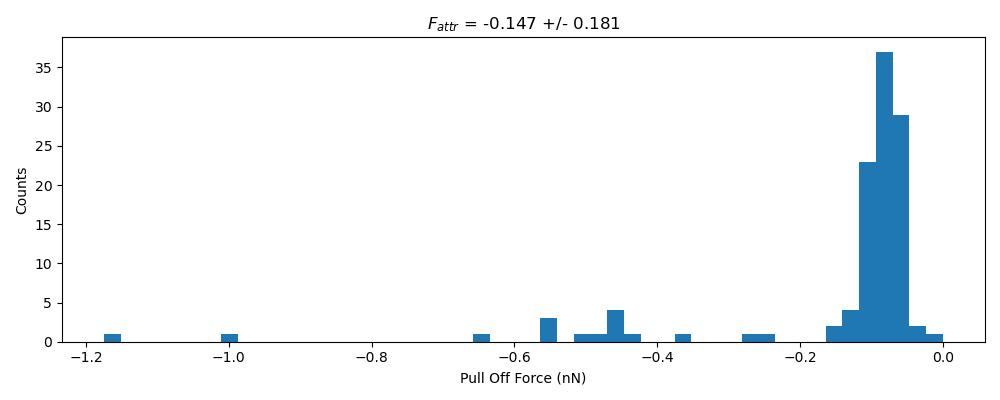
\includegraphics[width=\textwidth]{chapter7/Tip speed/5mM/S2 2Hz/retract_f_a_hist.jpg}
\caption{Retract curve for 5mM, S2 at 2Hz}
\end{figure}
\newpage


\begin{figure}[h!]
\paragraph{S3 2Hz}
\centering
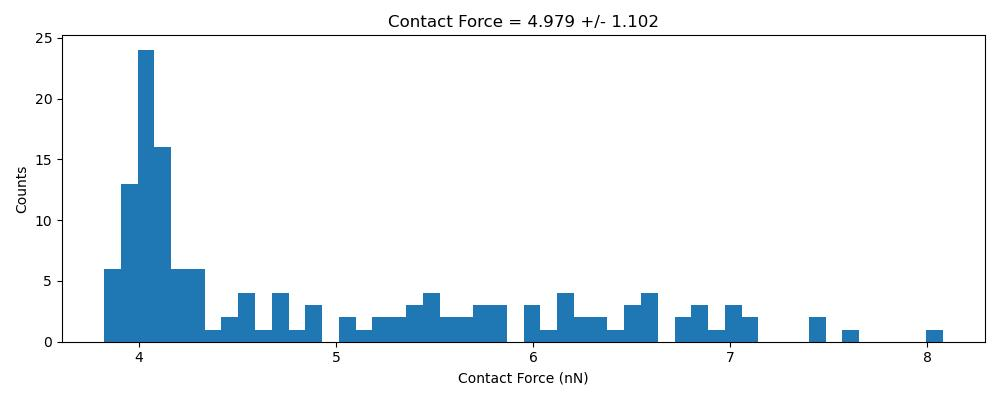
\includegraphics[width=\textwidth]{chapter7/Tip speed/5mM/S3 2Hz/approach_f_c_hist.jpg}
\caption{Approach curve for 5mM, S3 at 2Hz}
\end{figure}

\begin{figure}[h!]
\centering
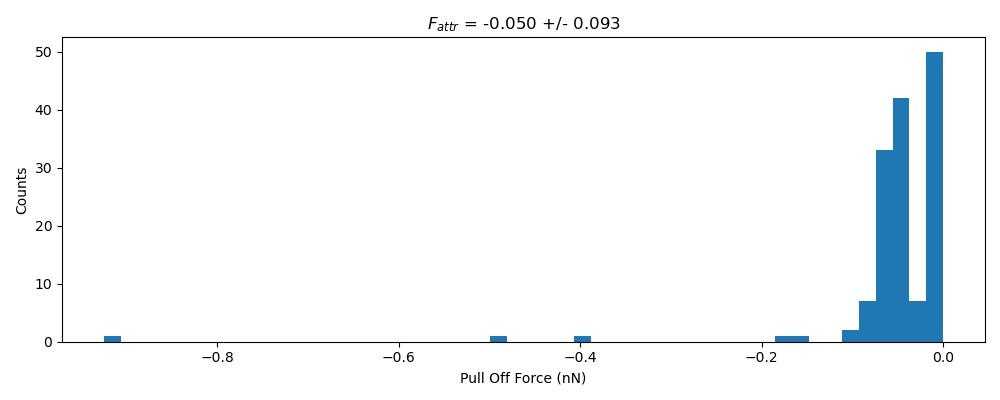
\includegraphics[width=\textwidth]{chapter7/Tip speed/5mM/S3 2Hz/retract_f_a_hist.jpg}
\caption{Retract curve for 5mM, S3 at 2Hz}
\end{figure}
\newpage

% 10mM Section
\subsubsection*{10mM}
10mM also includes an analysis of a slower tip - a tip speed of 0.1Hz. This was the only site to include a slower speed. Overall, for 0.1Hz, while 1 datapoint shows a significantly high attractive force, the other 2 largely show little to no attraction. Overall however, the 0.1Hz speed shows a slightly stronger retrace attractive force when compared to the previous data. 2Hz shows data within expected ranges from previous data.
\begin{figure}[h!]
\paragraph{S1 0.1Hz}
\centering
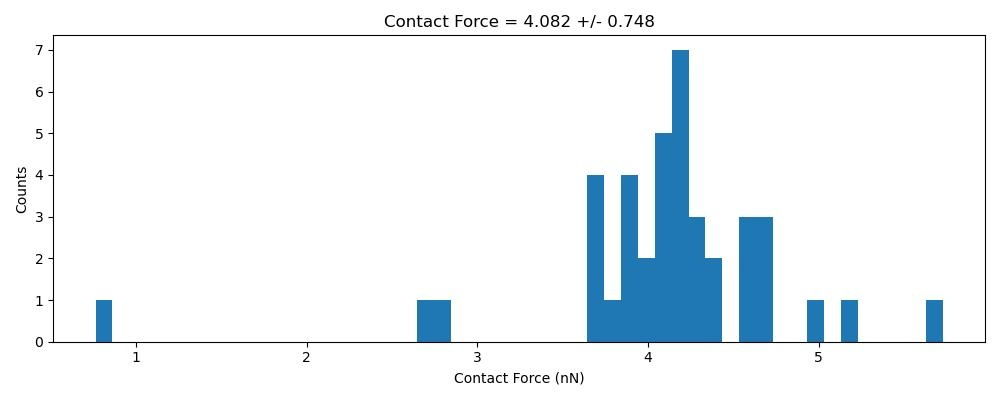
\includegraphics[width=\textwidth]{chapter7/Tip speed/10mM/S1 0.1Hz/approach_f_c_hist.jpg}
\caption{Approach curve for 10mM, S1 at 0.1Hz}
\end{figure}

\begin{figure}[h!]
\centering
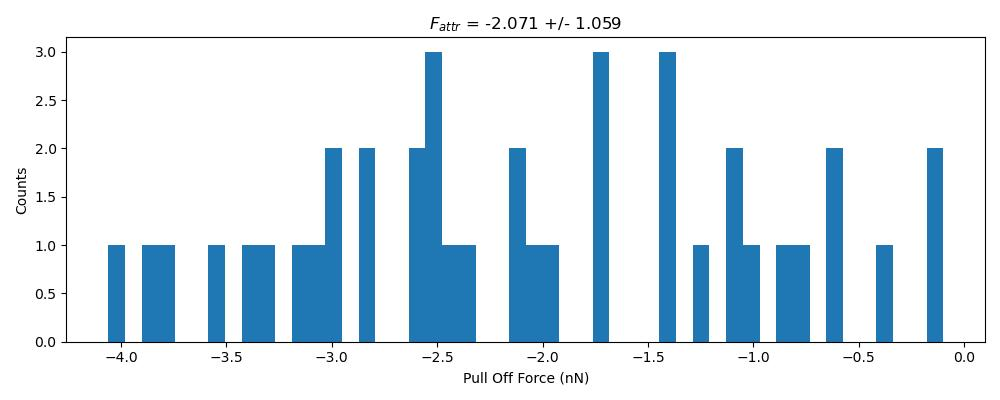
\includegraphics[width=\textwidth]{chapter7/Tip speed/10mM/S1 0.1Hz/retract_f_a_hist.jpg}
\caption{Retract curve for 10mM, S1 at 0.1Hz}
\end{figure}
\newpage

\begin{figure}[h!]
\paragraph{S1 2Hz}
\centering
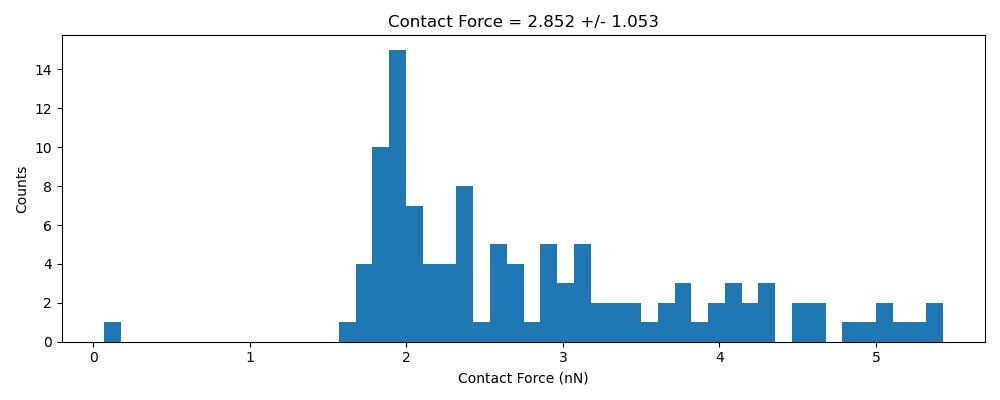
\includegraphics[width=\textwidth]{chapter7/Tip speed/10mM/S1 2Hz/approach_f_c_hist.jpg}
\caption{Approach curve for 10mM, S1 at 2Hz}
\end{figure}

\begin{figure}[h!]
\centering
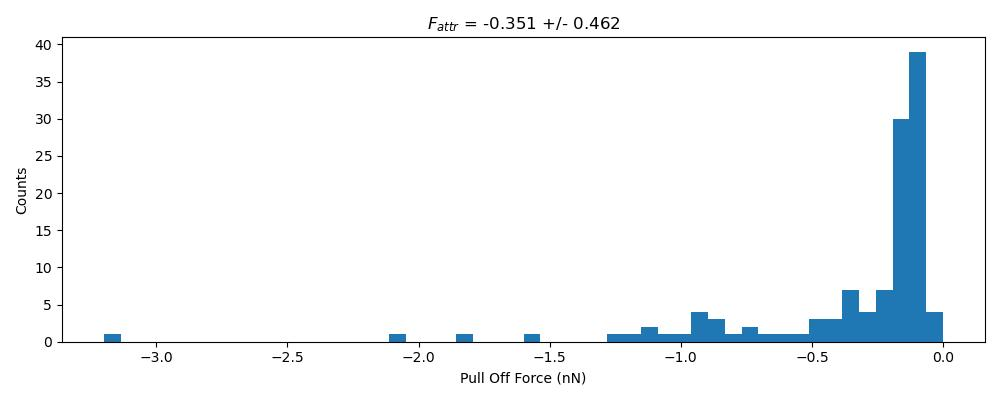
\includegraphics[width=\textwidth]{chapter7/Tip speed/10mM/S1 2Hz/retract_f_a_hist.jpg}
\caption{Retract curve for 10mM, S1 at 2Hz}
\end{figure}
\newpage


\begin{figure}[h!]
\paragraph{S2 0.1Hz}
\centering
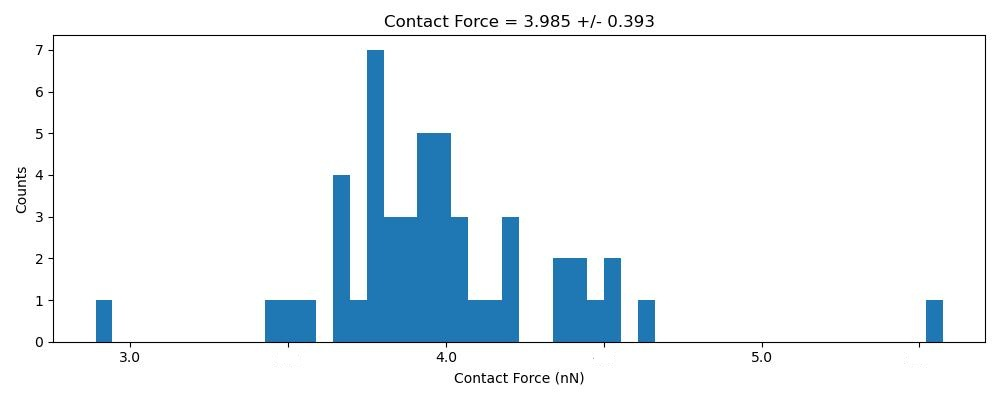
\includegraphics[width=\textwidth]{chapter7/Tip speed/10mM/S2 0.1Hz/approach_f_c_hist.jpg}
\caption{Approach curve for 10mM, S2 at 0.1Hz}
\end{figure}

\begin{figure}[h!]
\centering
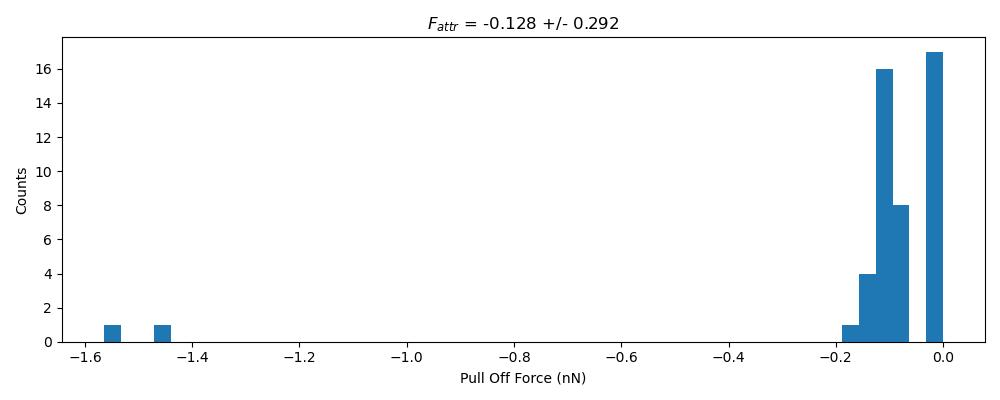
\includegraphics[width=\textwidth]{chapter7/Tip speed/10mM/S2 0.1Hz/retract_f_a_hist.jpg}
\caption{Retract curve for 10mM, S2 at 0.1Hz}
\end{figure}

\newpage


\begin{figure}[h!]
\paragraph{S2 2Hz}
\centering
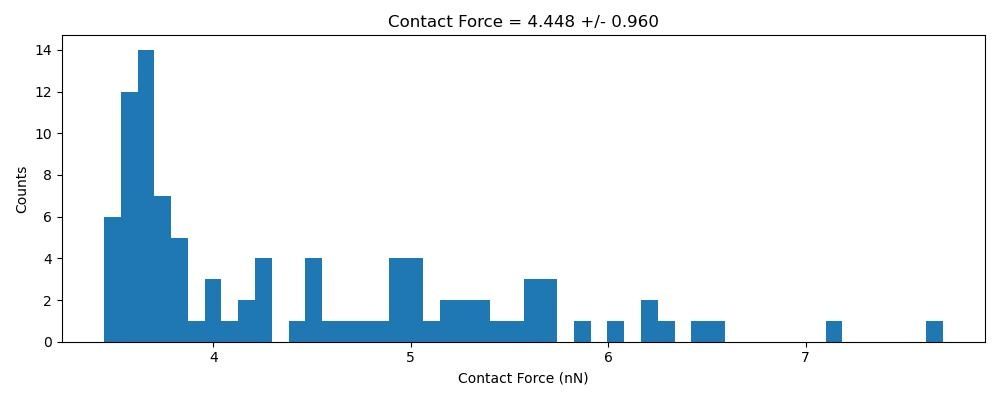
\includegraphics[width=\textwidth]{chapter7/Tip speed/10mM/S2 2Hz/approach_f_c_hist.jpg}
\caption{Approach curve for 10mM, S2 at 2Hz}
\end{figure}

\begin{figure}[h!]
\centering
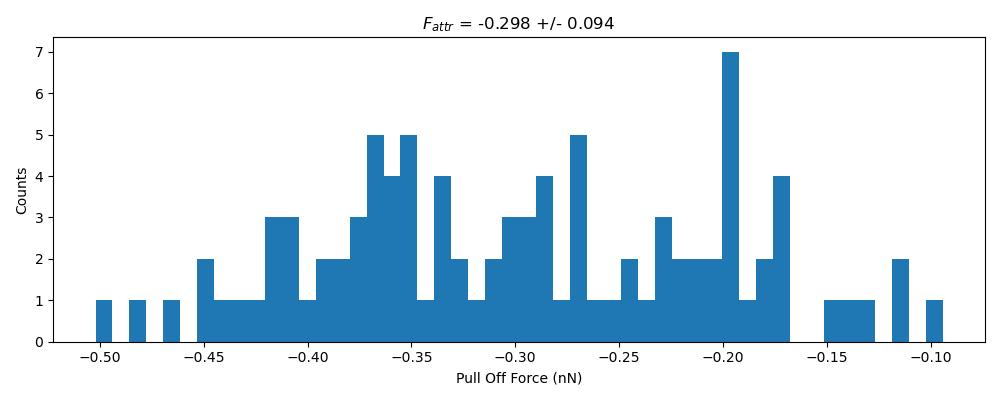
\includegraphics[width=\textwidth]{chapter7/Tip speed/10mM/S2 2Hz/retract_f_a_hist.jpg}
\caption{Retract curve for 10mM, S2 at 2Hz}
\end{figure}

\newpage


\begin{figure}[h!]
\paragraph{S3 0.1Hz}
\centering
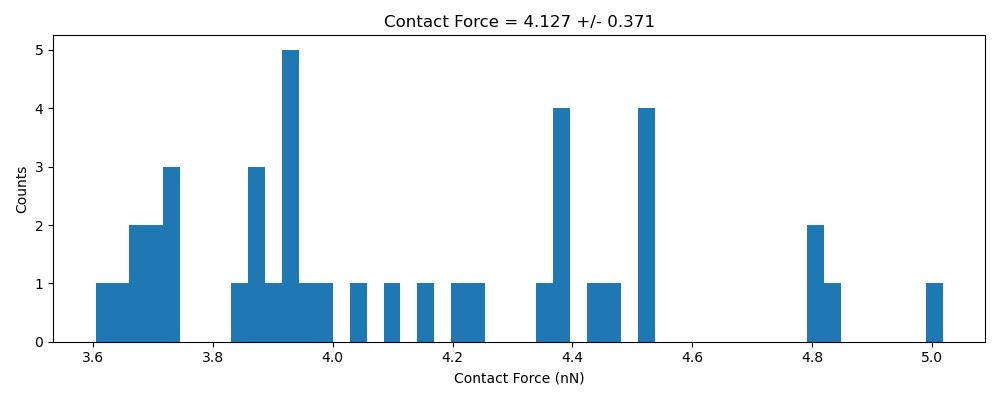
\includegraphics[width=\textwidth]{chapter7/Tip speed/10mM/S3 0.1Hz/approach_f_c_hist.jpg}
\caption{Approach curve for 10mM, S3 at 0.1Hz}
\end{figure}

\begin{figure}[h!]
\centering
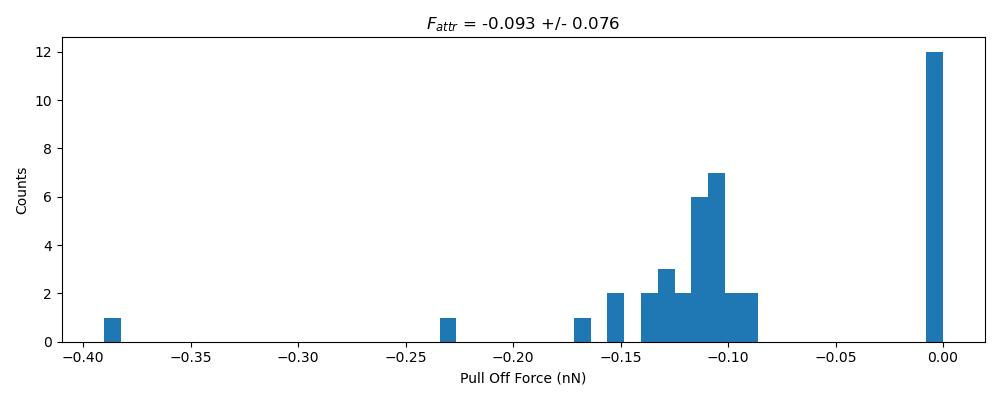
\includegraphics[width=\textwidth]{chapter7/Tip speed/10mM/S3 0.1Hz/retract_f_a_hist.jpg}
\caption{Retract curve for 10mM, S3 at 0.1Hz}
\end{figure}

\newpage


\begin{figure}[h!]
\paragraph{S3 2Hz}
\centering
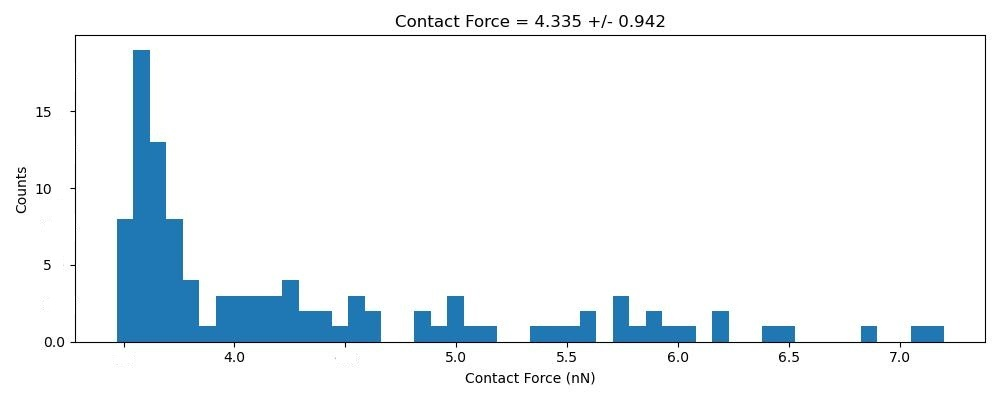
\includegraphics[width=\textwidth]{chapter7/Tip speed/10mM/S3 2Hz/approach_f_c_hist.jpg}
\caption{Approach curve for 10mM, S3 at 2Hz}
\end{figure}

\begin{figure}[h!]
\centering
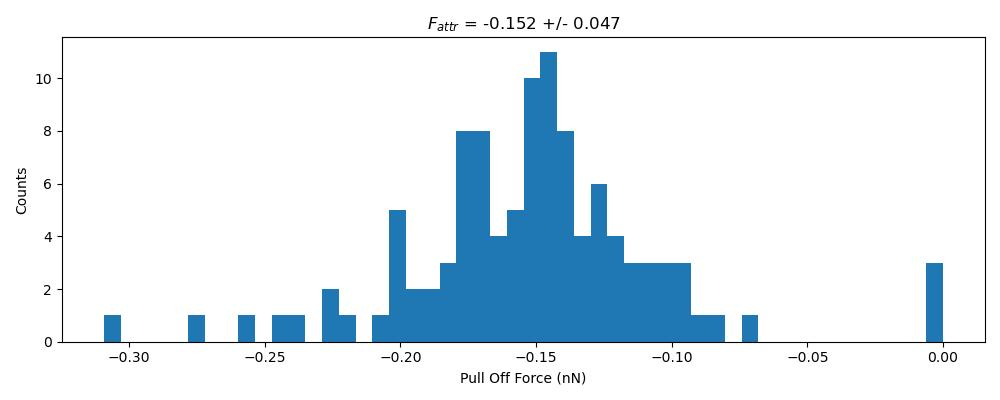
\includegraphics[width=\textwidth]{chapter7/Tip speed/10mM/S3 2Hz/retract_f_a_hist.jpg}
\caption{Retract curve for 10mM, S3 at 2Hz}
\end{figure}

\newpage

% 25mM Section
\subsubsection*{25mM}
25mM shows data within an expected range for the approach portion of the data, whereas the retrace demonstrates a significantly reduced attractive force. 
\begin{figure}[h!]
\paragraph{S1 2Hz}
\centering
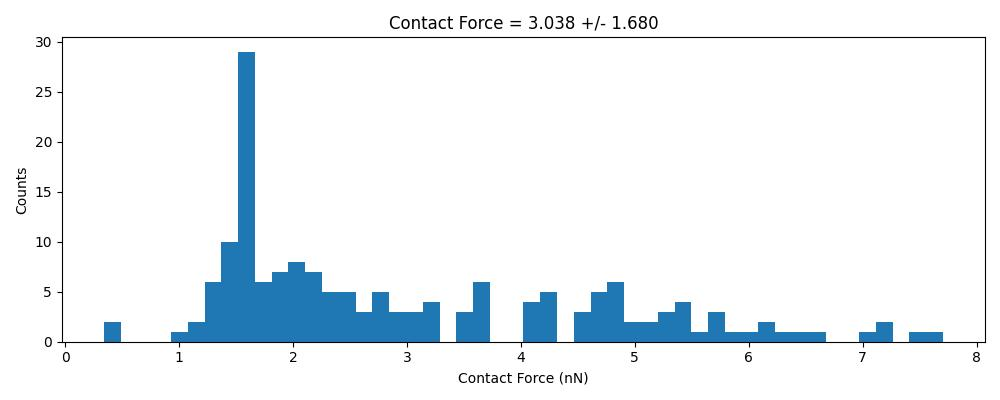
\includegraphics[width=\textwidth]{chapter7/Tip speed/25mM/S1 2Hz/approach_f_c_hist.jpg}
\caption{Approach curve for 25mM, S1 at 2Hz}
\end{figure}

\begin{figure}[h!]
\centering
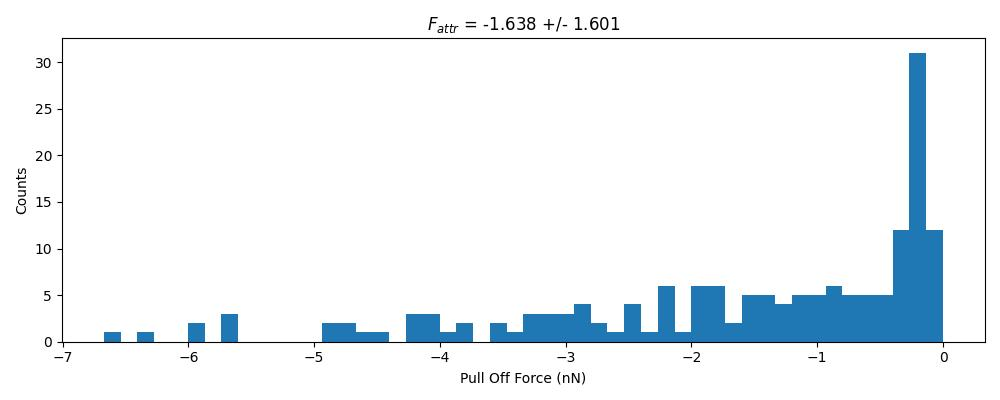
\includegraphics[width=\textwidth]{chapter7/Tip speed/25mM/S1 2Hz/retract_f_a_hist.jpg}
\caption{Retract curve for 25mM, S1 at 2Hz}
\end{figure}

\newpage


\begin{figure}[h!]
\paragraph{S2 2Hz}
\centering
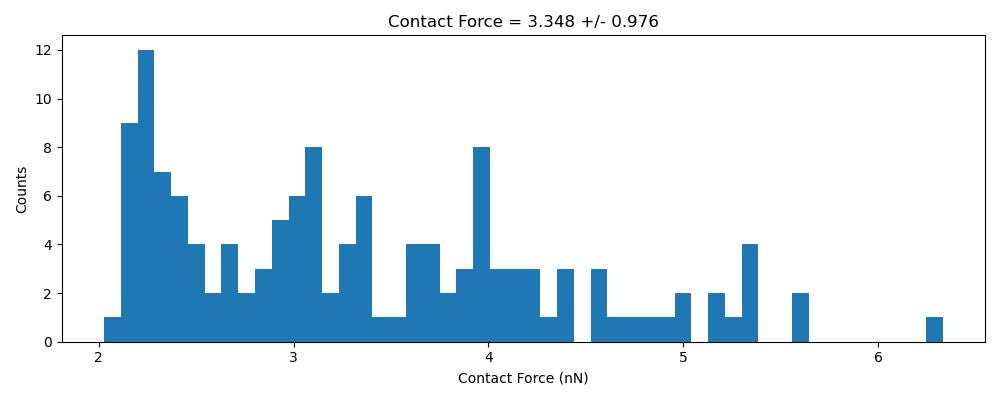
\includegraphics[width=\textwidth]{chapter7/Tip speed/25mM/S2 2Hz/approach_f_c_hist.jpg}
\caption{Approach curve for 25mM, S2 at 2Hz}
\end{figure}

\begin{figure}[h!]
\centering
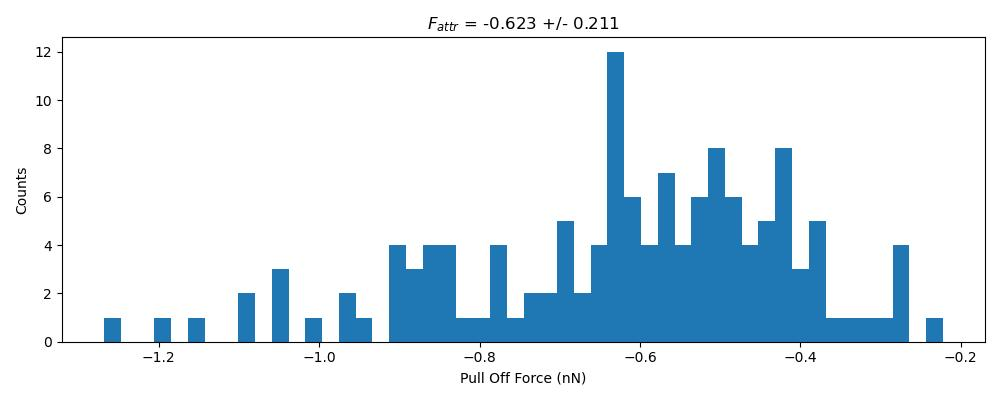
\includegraphics[width=\textwidth]{chapter7/Tip speed/25mM/S2 2Hz/retract_f_a_hist.jpg}
\caption{Retract curve for 25mM, S2 at 2Hz}
\end{figure}

\newpage


\begin{figure}[h!]
\paragraph{S3 2Hz}
\centering
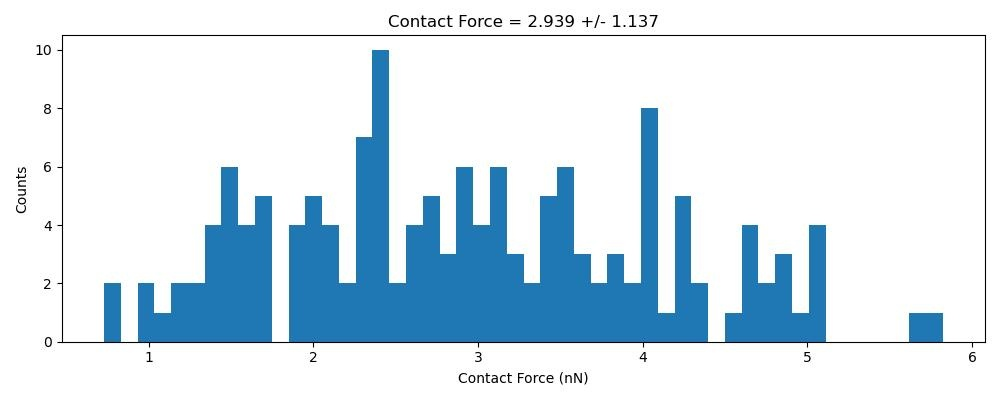
\includegraphics[width=\textwidth]{chapter7/Tip speed/25mM/S3 2Hz/approach_f_c_hist.jpg}
\caption{Approach curve for 25mM, S3 at 2Hz}
\end{figure}

\begin{figure}[h!]
\centering
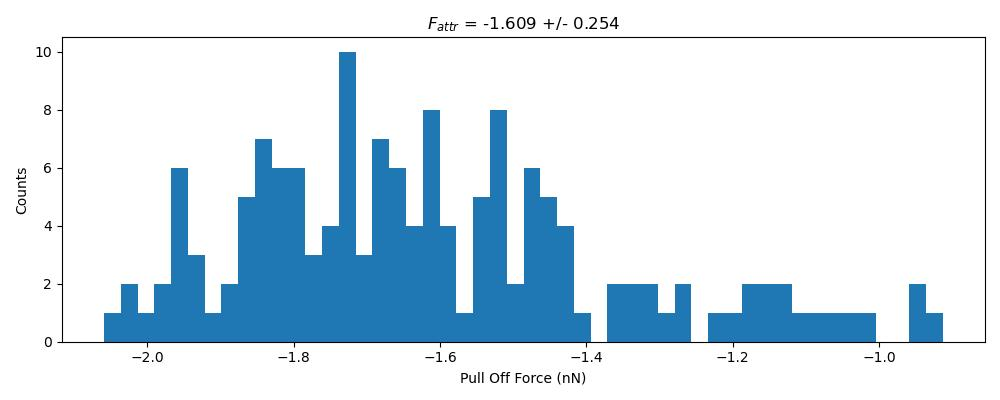
\includegraphics[width=\textwidth]{chapter7/Tip speed/25mM/S3 2Hz/retract_f_a_hist.jpg}
\caption{Retract curve for 25mM, S3 at 2Hz}
\end{figure}

\newpage

% 230mM Section
\subsubsection*{230mM}
230mM 2Hz again shows data within expected ranges, while having a slightly higher approach repulsive force. For the retrace attractive force, the results are similar, again with a slightly lower attractive force.
\begin{figure}[h!]
\paragraph{S1 2Hz}
\centering
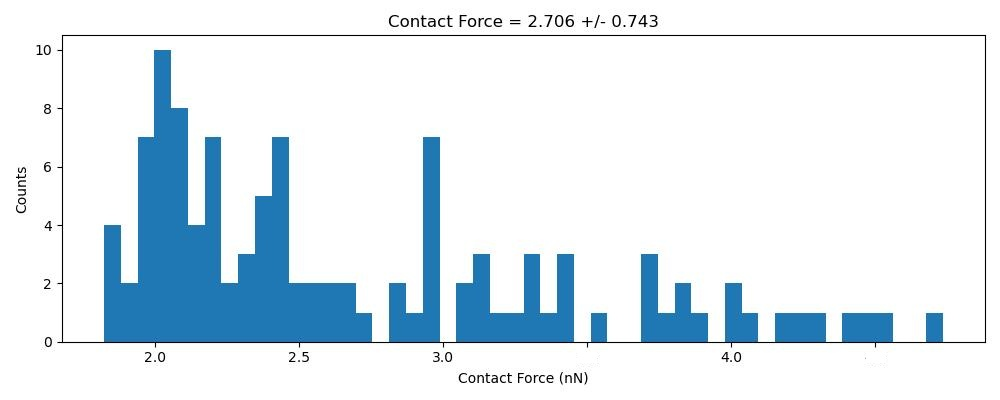
\includegraphics[width=\textwidth]{chapter7/Tip speed/230mM/S1 2Hz/approach_f_c_hist.jpg}
\caption{Approach curve for 230mM, S1 at 2Hz}
\end{figure}

\begin{figure}[h!]
\centering
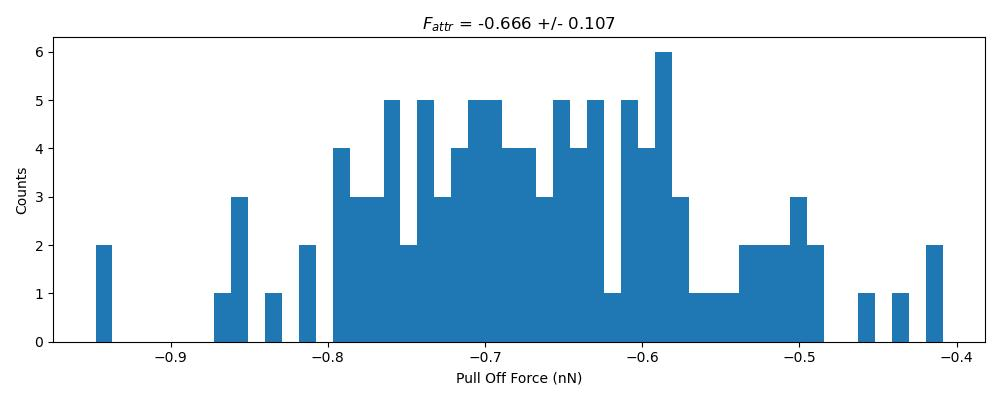
\includegraphics[width=\textwidth]{chapter7/Tip speed/230mM/S1 2Hz/retract_f_a_hist.jpg}
\caption{Retract curve for 230mM, S1 at 2Hz}
\end{figure}

\newpage


\begin{figure}[h!]
\paragraph{S2 2Hz}
\centering
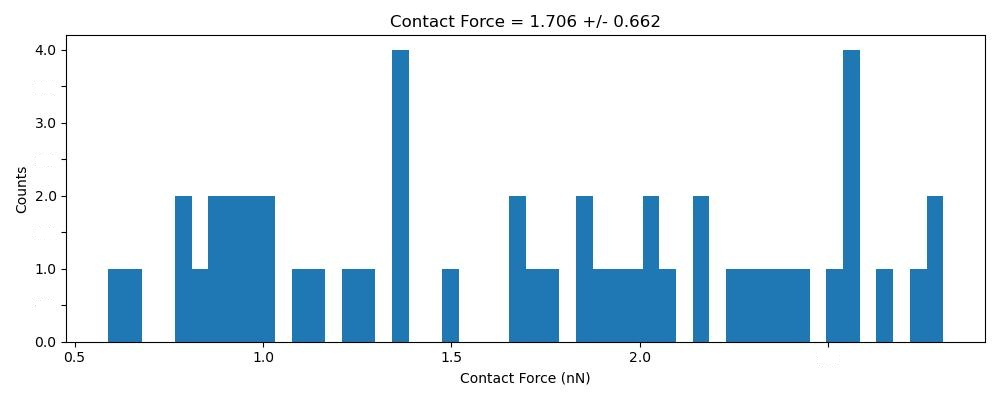
\includegraphics[width=\textwidth]{chapter7/Tip speed/230mM/S2 2Hz/approach_f_c_hist.jpg}
\caption{Approach curve for 230mM, S2 at 2Hz}
\end{figure}

\begin{figure}[h!]
\centering
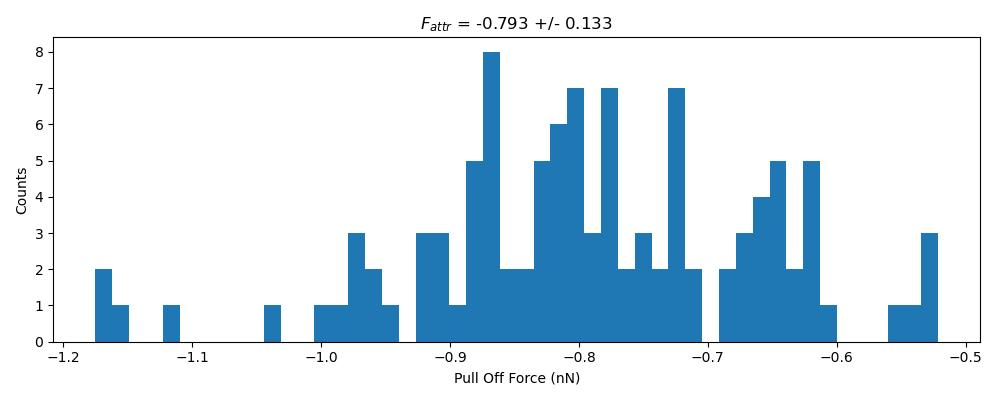
\includegraphics[width=\textwidth]{chapter7/Tip speed/230mM/S2 2Hz/retract_f_a_hist.jpg}
\caption{Retract curve for 230mM, S2 at 2Hz}
\end{figure}

\newpage

% 550mM Section
\subsubsection*{550mM}
550mM 2Hz marks a shift in approach forces towards the attractive. The results are similar again to other datapoints in this series; minorly reduced attractive force on the retrace. However, interestingly, the approach has very little attractive force. 
\begin{figure}[h!]
\paragraph{S2 2Hz}
\centering
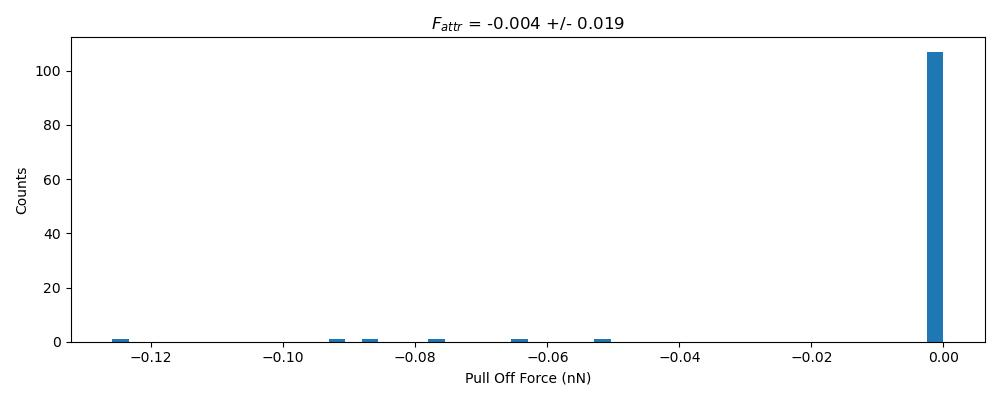
\includegraphics[width=\textwidth]{chapter7/Tip speed/550mM/S2 2Hz/approach_f_a_hist.jpg}
\caption{Approach curve for 550mM, S2 at 2Hz}
\end{figure}

\begin{figure}[h!]
\centering
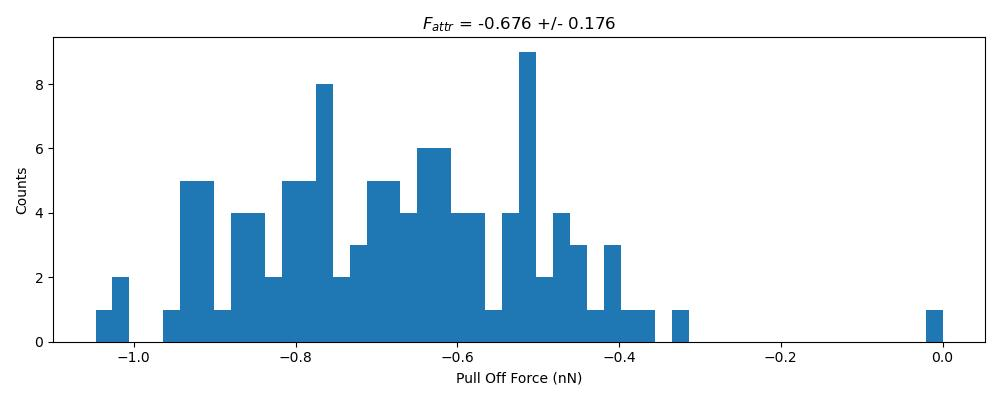
\includegraphics[width=\textwidth]{chapter7/Tip speed/550mM/S2 2Hz/retract_f_a_hist.jpg}
\caption{Retract curve for 550mM, S2 at 2Hz}
\end{figure}


\begin{figure}[h!]
\paragraph{S3 2Hz}
\centering
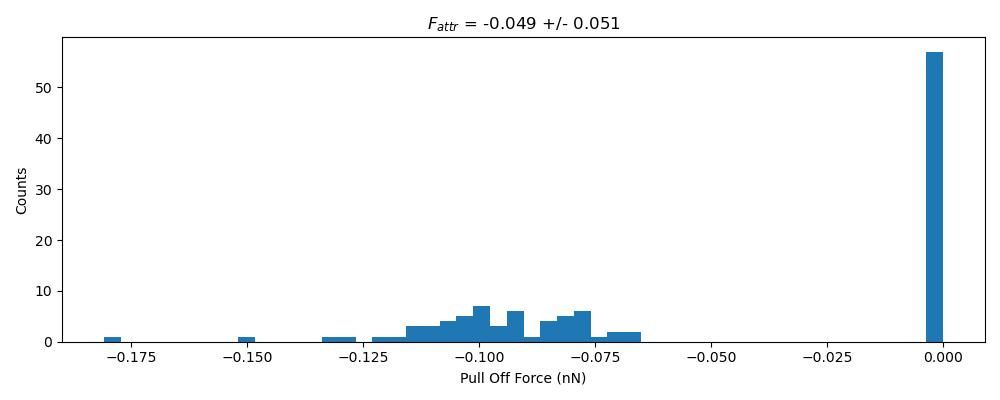
\includegraphics[width=\textwidth]{chapter7/Tip speed/550mM/S3 2Hz/approach_f_a_hist.jpg}
\caption{Approach curve for 550mM, S3 at 2Hz}
\end{figure}

\begin{figure}[h!]
\centering
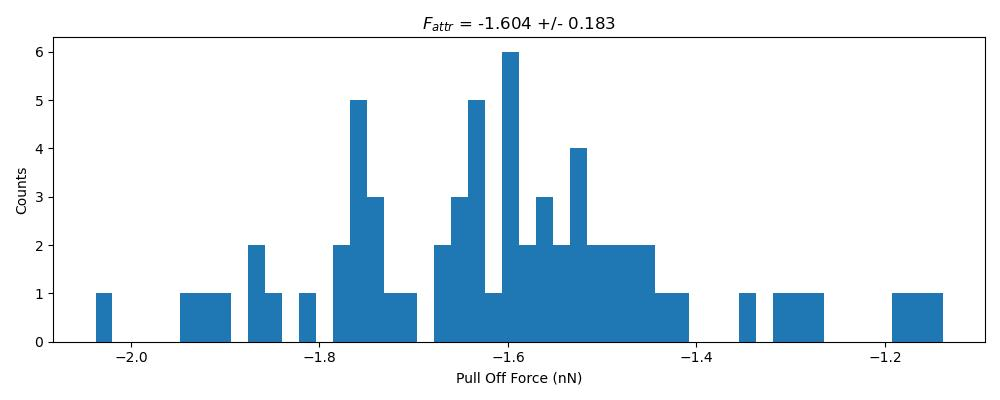
\includegraphics[width=\textwidth]{chapter7/Tip speed/550mM/S3 2Hz/retract_f_a_hist.jpg}
\caption{Retract curve for 550mM, S3 at 2Hz}
\end{figure}
